\documentclass[twoside]{book}

% Packages required by doxygen
\usepackage{fixltx2e}
\usepackage{calc}
\usepackage{doxygen}
\usepackage[export]{adjustbox} % also loads graphicx
\usepackage{graphicx}
\usepackage[utf8]{inputenc}
\usepackage{makeidx}
\usepackage{multicol}
\usepackage{multirow}
\PassOptionsToPackage{warn}{textcomp}
\usepackage{textcomp}
\usepackage[nointegrals]{wasysym}
\usepackage[table]{xcolor}

% Font selection
\usepackage[T1]{fontenc}
\usepackage[scaled=.90]{helvet}
\usepackage{courier}
\usepackage{amssymb}
\usepackage{sectsty}
\renewcommand{\familydefault}{\sfdefault}
\allsectionsfont{%
  \fontseries{bc}\selectfont%
  \color{darkgray}%
}
\renewcommand{\DoxyLabelFont}{%
  \fontseries{bc}\selectfont%
  \color{darkgray}%
}
\newcommand{\+}{\discretionary{\mbox{\scriptsize$\hookleftarrow$}}{}{}}

% Page & text layout
\usepackage{geometry}
\geometry{%
  a4paper,%
  top=2.5cm,%
  bottom=2.5cm,%
  left=2.5cm,%
  right=2.5cm%
}
\tolerance=750
\hfuzz=15pt
\hbadness=750
\setlength{\emergencystretch}{15pt}
\setlength{\parindent}{0cm}
\setlength{\parskip}{3ex plus 2ex minus 2ex}
\makeatletter
\renewcommand{\paragraph}{%
  \@startsection{paragraph}{4}{0ex}{-1.0ex}{1.0ex}{%
    \normalfont\normalsize\bfseries\SS@parafont%
  }%
}
\renewcommand{\subparagraph}{%
  \@startsection{subparagraph}{5}{0ex}{-1.0ex}{1.0ex}{%
    \normalfont\normalsize\bfseries\SS@subparafont%
  }%
}
\makeatother

% Headers & footers
\usepackage{fancyhdr}
\pagestyle{fancyplain}
\fancyhead[LE]{\fancyplain{}{\bfseries\thepage}}
\fancyhead[CE]{\fancyplain{}{}}
\fancyhead[RE]{\fancyplain{}{\bfseries\leftmark}}
\fancyhead[LO]{\fancyplain{}{\bfseries\rightmark}}
\fancyhead[CO]{\fancyplain{}{}}
\fancyhead[RO]{\fancyplain{}{\bfseries\thepage}}
\fancyfoot[LE]{\fancyplain{}{}}
\fancyfoot[CE]{\fancyplain{}{}}
\fancyfoot[RE]{\fancyplain{}{\bfseries\scriptsize Generated by Doxygen }}
\fancyfoot[LO]{\fancyplain{}{\bfseries\scriptsize Generated by Doxygen }}
\fancyfoot[CO]{\fancyplain{}{}}
\fancyfoot[RO]{\fancyplain{}{}}
\renewcommand{\footrulewidth}{0.4pt}
\renewcommand{\chaptermark}[1]{%
  \markboth{#1}{}%
}
\renewcommand{\sectionmark}[1]{%
  \markright{\thesection\ #1}%
}

% Indices & bibliography
\usepackage{natbib}
\usepackage[titles]{tocloft}
\setcounter{tocdepth}{3}
\setcounter{secnumdepth}{5}
\makeindex

% Hyperlinks (required, but should be loaded last)
\usepackage{ifpdf}
\ifpdf
  \usepackage[pdftex,pagebackref=true]{hyperref}
\else
  \usepackage[ps2pdf,pagebackref=true]{hyperref}
\fi
\hypersetup{%
  colorlinks=true,%
  linkcolor=blue,%
  citecolor=blue,%
  unicode%
}

% Custom commands
\newcommand{\clearemptydoublepage}{%
  \newpage{\pagestyle{empty}\cleardoublepage}%
}

\usepackage{caption}
\captionsetup{labelsep=space,justification=centering,font={bf},singlelinecheck=off,skip=4pt,position=top}

%===== C O N T E N T S =====

\begin{document}

% Titlepage & ToC
\hypersetup{pageanchor=false,
             bookmarksnumbered=true,
             pdfencoding=unicode
            }
\pagenumbering{alph}
\begin{titlepage}
\vspace*{7cm}
\begin{center}%
{\Large R\+PG Game \\[1ex]\large 2.\+0 }\\
\vspace*{1cm}
{\large Generated by Doxygen 1.8.13}\\
\end{center}
\end{titlepage}
\clearemptydoublepage
\pagenumbering{roman}
\tableofcontents
\clearemptydoublepage
\pagenumbering{arabic}
\hypersetup{pageanchor=true}

%--- Begin generated contents ---
\chapter{M\+S\+W\+\_\+\+Skywind\+\_\+\+Team}
\label{autotoc_md0}
\Hypertarget{autotoc_md0}
A programunk lényege, hogy kettő harcos párbaját leszimulálja. Ehhez létrehoztunk egy osztályt, amiből származtatunk két objektumot. Mindegyik harcosnak van neve, életerő pontja és sebzés pontja, melyeket az argumentumként megadott két txt fájlból nyer ki a program. A párbaj lezajlása\+: a harcosok felváltva támadják egymást, a támadott félnek pontosan annyival csökken az életerő pontja amennyi sebzés ponttal rendelkezik a támadó fél. A párbaj akkor ér véget, amikor az egyik félnek teljesen elfogynak az életerő pontjai.


\begin{DoxyItemize}
\item Linux rendszeren\+:
\begin{DoxyItemize}
\item Linux terminál megnyitása.
\item A \char`\"{}cd\char`\"{} parancs segítségével a programfájlokat tartalmazó mappába navigálás.
\item ./a.out és az ütköztetni kívánt két txt kiterjesztésű fájl megadása pl.\+: ./a.out Maple.\+txt Sally.\+txt
\item A txt fájlokban az alábbi példa szerint kell elhelyekedniük az adatoknak\+: \{ \char`\"{}name\char`\"{} \+: \char`\"{}\+Maple\char`\"{}, \char`\"{}hp\char`\"{} \+: 150, \char`\"{}dmg\char`\"{} \+: 10 \}
\end{DoxyItemize}
\item Windows rendszeren\+:
\begin{DoxyItemize}
\item A program futtatásához szükséges telepíteni egy Linux terminált (ajánlott program\+: \href{https://ubuntu.com/wsl}{\tt W\+SL Ubuntu})
\item A terminál feltelepítése után a program futtatásának menete megegyezik a \char`\"{}\+Linux rendszeren\char`\"{} menüpontban leírtakkal. 
\end{DoxyItemize}
\end{DoxyItemize}
\chapter{Hierarchical Index}
\section{Class Hierarchy}
This inheritance list is sorted roughly, but not completely, alphabetically\+:\begin{DoxyCompactList}
\item exception\begin{DoxyCompactList}
\item \contentsline{section}{J\+S\+ON\+:\+:Parse\+Exception}{\pageref{classJSON_1_1ParseException}}{}
\end{DoxyCompactList}
\item \contentsline{section}{J\+S\+ON}{\pageref{classJSON}}{}
\item \contentsline{section}{Monster}{\pageref{classMonster}}{}
\begin{DoxyCompactList}
\item \contentsline{section}{Hero}{\pageref{classHero}}{}
\end{DoxyCompactList}
\end{DoxyCompactList}

\chapter{Class Index}
\doxysection{Class List}
Here are the classes, structs, unions and interfaces with brief descriptions\+:\begin{DoxyCompactList}
\item\contentsline{section}{\mbox{\hyperlink{classHero}{Hero}} }{\pageref{classHero}}{}
\item\contentsline{section}{\mbox{\hyperlink{classJSON}{J\+S\+ON}} }{\pageref{classJSON}}{}
\item\contentsline{section}{\mbox{\hyperlink{classMonster}{Monster}} }{\pageref{classMonster}}{}
\item\contentsline{section}{\mbox{\hyperlink{classJSON_1_1ParseException}{J\+S\+O\+N\+::\+Parse\+Exception}} }{\pageref{classJSON_1_1ParseException}}{}
\end{DoxyCompactList}

\chapter{Class Documentation}
\hypertarget{classHero}{}\section{Hero Class Reference}
\label{classHero}\index{Hero@{Hero}}


{\ttfamily \#include $<$Hero.\+h$>$}



Inheritance diagram for Hero\+:
\nopagebreak
\begin{figure}[H]
\begin{center}
\leavevmode
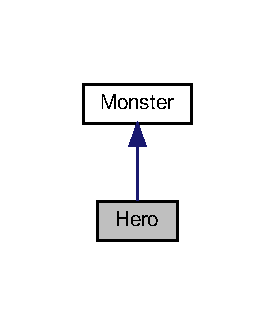
\includegraphics[width=132pt]{classHero__inherit__graph}
\end{center}
\end{figure}


Collaboration diagram for Hero\+:
\nopagebreak
\begin{figure}[H]
\begin{center}
\leavevmode
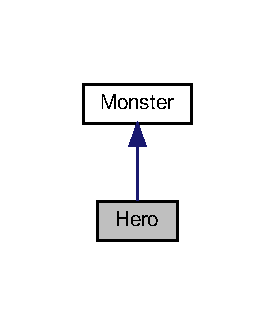
\includegraphics[width=132pt]{classHero__coll__graph}
\end{center}
\end{figure}
\subsection*{Public Member Functions}
\begin{DoxyCompactItemize}
\item 
\mbox{\Hypertarget{classHero_a2b2487de5bea68a17d535e8155c0d99a}\label{classHero_a2b2487de5bea68a17d535e8155c0d99a}} 
\hyperlink{classHero_a2b2487de5bea68a17d535e8155c0d99a}{Hero} (const std\+::string, int, int, float, const int, const int, const int, const float)
\begin{DoxyCompactList}\small\item\em A \hyperlink{classHero}{Hero} konstruktora. A \hyperlink{classHero}{Hero} létrehozásakor paraméterként megadott értékekkel ruházza fel a Hero-\/t. (name, hp, dmg, attackcooldown, exp\+Per\+Lvl, hp\+Bonus, dmg\+Bonus, attack\+Cd\+Mp) \end{DoxyCompactList}\item 
\mbox{\Hypertarget{classHero_aca45aa10e1caefaf84a22ed42fd4f7df}\label{classHero_aca45aa10e1caefaf84a22ed42fd4f7df}} 
int \hyperlink{classHero_aca45aa10e1caefaf84a22ed42fd4f7df}{get\+Exp} () const
\begin{DoxyCompactList}\small\item\em Exp lekérő metódus. Visszaadja, hogy mennyi tapasztalati ponttal rendelkezik a \hyperlink{classHero}{Hero}. \end{DoxyCompactList}\item 
\mbox{\Hypertarget{classHero_a17e77f3769e62aeb4e1807bbfc720f47}\label{classHero_a17e77f3769e62aeb4e1807bbfc720f47}} 
int \hyperlink{classHero_a17e77f3769e62aeb4e1807bbfc720f47}{get\+Level} () const
\begin{DoxyCompactList}\small\item\em Szint lekérő metódus. Visszaadja a \hyperlink{classHero}{Hero} szintjét. \end{DoxyCompactList}\item 
\mbox{\Hypertarget{classHero_ac6a7deeb6e390a23536d622042f4c48e}\label{classHero_ac6a7deeb6e390a23536d622042f4c48e}} 
int \hyperlink{classHero_ac6a7deeb6e390a23536d622042f4c48e}{get\+Max\+Health\+Points} () const
\begin{DoxyCompactList}\small\item\em Maximum élererőpont lekérő metódus. Visszaadja a \hyperlink{classHero}{Hero} maximum élererőpontját. \end{DoxyCompactList}\item 
void \hyperlink{classHero_a367347243a9066b06ccfc766dbac6e56}{set\+Dmg} (int)
\begin{DoxyCompactList}\small\item\em Sebzéspont beállító metódus. Beállítja a \hyperlink{classHero}{Hero} sebzéspontját a paraméterként megadott értékre. \end{DoxyCompactList}\item 
void \hyperlink{classHero_a1cc85148b78583aa9dbad3bc5aff140c}{set\+Attack\+Cd} (float)
\begin{DoxyCompactList}\small\item\em Attackcooldown beállító metódus. Beállítja a \hyperlink{classHero}{Hero} támadásának betöltési idejét a paraméterként megadott értékre. \end{DoxyCompactList}\item 
\mbox{\Hypertarget{classHero_ade2f8025cdd571870f5855567a1058b9}\label{classHero_ade2f8025cdd571870f5855567a1058b9}} 
void \hyperlink{classHero_ade2f8025cdd571870f5855567a1058b9}{mod\+Datas} ()
\begin{DoxyCompactList}\small\item\em Adatmódosító metódus. A \hyperlink{classHero}{Hero} szintlépésével járó adatokat változtatja meg. \end{DoxyCompactList}\item 
void \hyperlink{classHero_a4c2c5bcf53b4fa4cb931d9930e3f0844}{Attack} (\hyperlink{classMonster}{Monster} $\ast$) override
\begin{DoxyCompactList}\small\item\em Attack metódus. A függvényt meghívó \hyperlink{classHero}{Hero} megtámadja a paraméterben megadott Monster-\/t, így a paraméterben megadott \hyperlink{classMonster}{Monster} életerőpontját csökkenti a hívó \hyperlink{classHero}{Hero} sebzéspontjával, feltéve, ha az adott \hyperlink{classMonster}{Monster} még kibír ekkora támadást, ha nem akkor a védekező fél életerpontját 0-\/ra állítja továbbá gondoskodik, hogy a \hyperlink{classHero}{Hero} megkapja a neki járó tapasztalatot és az ennek köszönhető szinteket. \end{DoxyCompactList}\item 
\mbox{\Hypertarget{classHero_a5aeef41ede5a80dc29c5acd7b553c4da}\label{classHero_a5aeef41ede5a80dc29c5acd7b553c4da}} 
\hyperlink{classHero_a5aeef41ede5a80dc29c5acd7b553c4da}{$\sim$\+Hero} ()
\begin{DoxyCompactList}\small\item\em A \hyperlink{classHero}{Hero} osztály destruktora. \end{DoxyCompactList}\end{DoxyCompactItemize}
\subsection*{Static Public Member Functions}
\begin{DoxyCompactItemize}
\item 
\mbox{\Hypertarget{classHero_ae2281a5142355d85b799cc836cd90bcf}\label{classHero_ae2281a5142355d85b799cc836cd90bcf}} 
static \hyperlink{classHero}{Hero} \hyperlink{classHero_ae2281a5142355d85b799cc836cd90bcf}{parse} (std\+::string)
\begin{DoxyCompactList}\small\item\em parse metódus. A paraméterként megadott fájlból kinyeri a \hyperlink{classHero}{Hero} létrehozásához szükséges adatokat majd létrehozza és vissza is tér vele. \end{DoxyCompactList}\end{DoxyCompactItemize}
\subsection*{Additional Inherited Members}


\subsection{Detailed Description}
A \hyperlink{classHero}{Hero} adatait és metódusait tartalmazó class

\begin{DoxyAuthor}{Authors}
Daniel\+Zettis, kormendiakos, M\+Zsolt97
\end{DoxyAuthor}
\begin{DoxyVersion}{Version}
2.\+0
\end{DoxyVersion}
\begin{DoxyDate}{Date}
2020/11/06
\end{DoxyDate}
Létrehozva\+: 2020/11/06 

\subsection{Member Function Documentation}
\mbox{\Hypertarget{classHero_a4c2c5bcf53b4fa4cb931d9930e3f0844}\label{classHero_a4c2c5bcf53b4fa4cb931d9930e3f0844}} 
\index{Hero@{Hero}!Attack@{Attack}}
\index{Attack@{Attack}!Hero@{Hero}}
\subsubsection{\texorpdfstring{Attack()}{Attack()}}
{\footnotesize\ttfamily void Hero\+::\+Attack (\begin{DoxyParamCaption}\item[{\hyperlink{classMonster}{Monster} $\ast$}]{m }\end{DoxyParamCaption})\hspace{0.3cm}{\ttfamily [override]}, {\ttfamily [virtual]}}



Attack metódus. A függvényt meghívó \hyperlink{classHero}{Hero} megtámadja a paraméterben megadott Monster-\/t, így a paraméterben megadott \hyperlink{classMonster}{Monster} életerőpontját csökkenti a hívó \hyperlink{classHero}{Hero} sebzéspontjával, feltéve, ha az adott \hyperlink{classMonster}{Monster} még kibír ekkora támadást, ha nem akkor a védekező fél életerpontját 0-\/ra állítja továbbá gondoskodik, hogy a \hyperlink{classHero}{Hero} megkapja a neki járó tapasztalatot és az ennek köszönhető szinteket. 


\begin{DoxyParams}[1]{Parameters}
\mbox{\tt in}  & {\em m} & A megtámadni kívánt \hyperlink{classMonster}{Monster} memóriacíme. \\
\hline
\end{DoxyParams}


Reimplemented from \hyperlink{classMonster_a8de70695e71755873f1f3cc0c78ef549}{Monster}.

\mbox{\Hypertarget{classHero_a1cc85148b78583aa9dbad3bc5aff140c}\label{classHero_a1cc85148b78583aa9dbad3bc5aff140c}} 
\index{Hero@{Hero}!set\+Attack\+Cd@{set\+Attack\+Cd}}
\index{set\+Attack\+Cd@{set\+Attack\+Cd}!Hero@{Hero}}
\subsubsection{\texorpdfstring{set\+Attack\+Cd()}{setAttackCd()}}
{\footnotesize\ttfamily void Hero\+::set\+Attack\+Cd (\begin{DoxyParamCaption}\item[{float}]{attack\+Cd\+\_\+ }\end{DoxyParamCaption})}



Attackcooldown beállító metódus. Beállítja a \hyperlink{classHero}{Hero} támadásának betöltési idejét a paraméterként megadott értékre. 


\begin{DoxyParams}[1]{Parameters}
\mbox{\tt in}  & {\em attack\+Cd\+\_\+} & A beállítani kívánt érték \\
\hline
\end{DoxyParams}
\mbox{\Hypertarget{classHero_a367347243a9066b06ccfc766dbac6e56}\label{classHero_a367347243a9066b06ccfc766dbac6e56}} 
\index{Hero@{Hero}!set\+Dmg@{set\+Dmg}}
\index{set\+Dmg@{set\+Dmg}!Hero@{Hero}}
\subsubsection{\texorpdfstring{set\+Dmg()}{setDmg()}}
{\footnotesize\ttfamily void Hero\+::set\+Dmg (\begin{DoxyParamCaption}\item[{int}]{dmg\+\_\+ }\end{DoxyParamCaption})}



Sebzéspont beállító metódus. Beállítja a \hyperlink{classHero}{Hero} sebzéspontját a paraméterként megadott értékre. 


\begin{DoxyParams}[1]{Parameters}
\mbox{\tt in}  & {\em dmg\+\_\+} & A beállítani kívánt érték \\
\hline
\end{DoxyParams}


The documentation for this class was generated from the following files\+:\begin{DoxyCompactItemize}
\item 
Hero.\+h\item 
Hero.\+cpp\end{DoxyCompactItemize}

\hypertarget{classJSON}{}\section{J\+S\+ON Class Reference}
\label{classJSON}\index{J\+S\+ON@{J\+S\+ON}}


{\ttfamily \#include $<$J\+S\+O\+N.\+h$>$}

\subsection*{Classes}
\begin{DoxyCompactItemize}
\item 
class \hyperlink{classJSON_1_1ParseException}{Parse\+Exception}
\end{DoxyCompactItemize}
\subsection*{Public Member Functions}
\begin{DoxyCompactItemize}
\item 
\mbox{\Hypertarget{classJSON_aba4f484f3ee84128f50ffd4d3b20ccf1}\label{classJSON_aba4f484f3ee84128f50ffd4d3b20ccf1}} 
\hyperlink{classJSON_aba4f484f3ee84128f50ffd4d3b20ccf1}{J\+S\+ON} (const std\+::map$<$ std\+::string, std\+::any $>$ \&)
\begin{DoxyCompactList}\small\item\em A \hyperlink{classJSON}{J\+S\+ON} konstruktora. A \hyperlink{classJSON}{J\+S\+ON} létrehozásához egy map-\/ot vár. \end{DoxyCompactList}\item 
\mbox{\Hypertarget{classJSON_a6e05c25394240770da452ee6c13ed5bf}\label{classJSON_a6e05c25394240770da452ee6c13ed5bf}} 
{\footnotesize template$<$typename T $>$ }\\T \hyperlink{classJSON_a6e05c25394240770da452ee6c13ed5bf}{get} (std\+::string key)
\begin{DoxyCompactList}\small\item\em get metódus. Visszaadja a paraméterként megadott kulcshoz rendelt értéket egy map-\/ből. \end{DoxyCompactList}\item 
\mbox{\Hypertarget{classJSON_a896544dd87ac36e8d8e4137f51ade9c2}\label{classJSON_a896544dd87ac36e8d8e4137f51ade9c2}} 
int \hyperlink{classJSON_a896544dd87ac36e8d8e4137f51ade9c2}{count} (std\+::string key)
\begin{DoxyCompactList}\small\item\em count metódus. Megszámolja, hogy a paranéterként adott kulcs hányszor szerepel a map-\/ben. 0 vagy 1 lehet 0, ha nincs a map-\/ben, 1, ha van \end{DoxyCompactList}\item 
\mbox{\Hypertarget{classJSON_ad21d0848fcee452fe2434c653bc87510}\label{classJSON_ad21d0848fcee452fe2434c653bc87510}} 
\hyperlink{classJSON_ad21d0848fcee452fe2434c653bc87510}{$\sim$\+J\+S\+ON} ()
\begin{DoxyCompactList}\small\item\em A \hyperlink{classJSON}{J\+S\+ON} osztály destruktora. \end{DoxyCompactList}\end{DoxyCompactItemize}
\subsection*{Static Public Member Functions}
\begin{DoxyCompactItemize}
\item 
\mbox{\Hypertarget{classJSON_a13577194c8ba3bfb544168f306a33f83}\label{classJSON_a13577194c8ba3bfb544168f306a33f83}} 
static std\+::string \hyperlink{classJSON_a13577194c8ba3bfb544168f306a33f83}{input\+File} (std\+::string)
\begin{DoxyCompactList}\small\item\em input\+File metódus. Megnyitja a paraméterként megadott fájlt és betölti a tartalmát egy stringbe, minden betöltött string után egy szóközt téve. \end{DoxyCompactList}\item 
\mbox{\Hypertarget{classJSON_a196e7e19e4a6d762cddda6dd71237a63}\label{classJSON_a196e7e19e4a6d762cddda6dd71237a63}} 
static std\+::string \hyperlink{classJSON_a196e7e19e4a6d762cddda6dd71237a63}{data\+From\+File} (std\+::string, std\+::string)
\begin{DoxyCompactList}\small\item\em data\+From\+File metódus. Az első paraméterként megadott stringből, kinyeri, majd visszaadja a második paraméterként megadott kulcshoz tartozó értéket. \end{DoxyCompactList}\item 
\mbox{\Hypertarget{classJSON_a88b145f10f9784da452b895bc327f358}\label{classJSON_a88b145f10f9784da452b895bc327f358}} 
static \hyperlink{classJSON}{J\+S\+ON} \hyperlink{classJSON_a88b145f10f9784da452b895bc327f358}{parse\+From\+File} (std\+::string)
\begin{DoxyCompactList}\small\item\em parse\+From\+File metódus. A paraméterként megadott fájlból kinyeri a Hero-\/t és a \hyperlink{classMonster}{Monster(eke)}t és eltárolja őket egy mapben, amellyel létrehoz egy \hyperlink{classJSON}{J\+S\+ON} objektumot és visszatér vele. \end{DoxyCompactList}\end{DoxyCompactItemize}
\subsection*{Protected Attributes}
\begin{DoxyCompactItemize}
\item 
\mbox{\Hypertarget{classJSON_a017be2f0262f19e399ba1e86b9a5144a}\label{classJSON_a017be2f0262f19e399ba1e86b9a5144a}} 
std\+::map$<$ std\+::string, std\+::any $>$ \hyperlink{classJSON_a017be2f0262f19e399ba1e86b9a5144a}{map}
\begin{DoxyCompactList}\small\item\em A Hero-\/t és a \hyperlink{classMonster}{Monster(eke)}t tartalmazó map. \end{DoxyCompactList}\end{DoxyCompactItemize}


\subsection{Detailed Description}
A \hyperlink{classJSON}{J\+S\+ON} adatait és metódusait tartalmazó class

\begin{DoxyAuthor}{Authors}
Daniel\+Zettis, kormendiakos, M\+Zsolt97
\end{DoxyAuthor}
\begin{DoxyVersion}{Version}
2.\+0
\end{DoxyVersion}
\begin{DoxyDate}{Date}
2020/11/06
\end{DoxyDate}
Létrehozva\+: 2020/11/06 

The documentation for this class was generated from the following files\+:\begin{DoxyCompactItemize}
\item 
J\+S\+O\+N.\+h\item 
J\+S\+O\+N.\+cpp\end{DoxyCompactItemize}

\hypertarget{classMonster}{}\doxysection{Monster Class Reference}
\label{classMonster}\index{Monster@{Monster}}


{\ttfamily \#include $<$Monster.\+h$>$}



Inheritance diagram for Monster\+:
\nopagebreak
\begin{figure}[H]
\begin{center}
\leavevmode
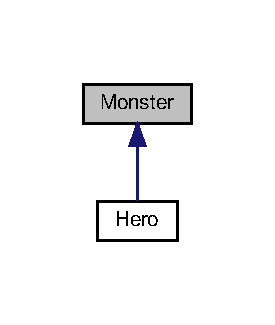
\includegraphics[width=136pt]{classMonster__inherit__graph}
\end{center}
\end{figure}
\doxysubsection*{Public Member Functions}
\begin{DoxyCompactItemize}
\item 
\mbox{\Hypertarget{classMonster_abc26caf327967646c0b9fce3b231c410}\label{classMonster_abc26caf327967646c0b9fce3b231c410}} 
\mbox{\hyperlink{classMonster_abc26caf327967646c0b9fce3b231c410}{Monster}} (const std\+::string, int, int, float)
\begin{DoxyCompactList}\small\item\em A \mbox{\hyperlink{classMonster}{Monster}} konstruktora. A \mbox{\hyperlink{classMonster}{Monster}} létrehozásakor paraméterként megadott értékekkel ruházza fel a Monster-\/t. (name, hp, dmg, attackcooldown) \end{DoxyCompactList}\item 
\mbox{\Hypertarget{classMonster_a28ae1112e37262ce150e3c02465b3dd5}\label{classMonster_a28ae1112e37262ce150e3c02465b3dd5}} 
std\+::string \mbox{\hyperlink{classMonster_a28ae1112e37262ce150e3c02465b3dd5}{get\+Name}} () const
\begin{DoxyCompactList}\small\item\em Név lekérő metódus. Visszaadja a \mbox{\hyperlink{classMonster}{Monster}} nevét. \end{DoxyCompactList}\item 
\mbox{\Hypertarget{classMonster_acbfb552014439fe02d10f2492e60fe34}\label{classMonster_acbfb552014439fe02d10f2492e60fe34}} 
int \mbox{\hyperlink{classMonster_acbfb552014439fe02d10f2492e60fe34}{get\+Health\+Points}} () const
\begin{DoxyCompactList}\small\item\em Életerőpont lekérő metódus. Visszaadja a \mbox{\hyperlink{classMonster}{Monster}} életerőpontját. \end{DoxyCompactList}\item 
\mbox{\Hypertarget{classMonster_a5872e19f684e0a81ead15da3e82992ad}\label{classMonster_a5872e19f684e0a81ead15da3e82992ad}} 
int \mbox{\hyperlink{classMonster_a5872e19f684e0a81ead15da3e82992ad}{get\+Damage}} () const
\begin{DoxyCompactList}\small\item\em Sebzéspont lekérő metódus. Visszaadja a \mbox{\hyperlink{classMonster}{Monster}} sebzéspontját. \end{DoxyCompactList}\item 
\mbox{\Hypertarget{classMonster_abcb5bbbf0cd0ff5c599438511a63a6ae}\label{classMonster_abcb5bbbf0cd0ff5c599438511a63a6ae}} 
float \mbox{\hyperlink{classMonster_abcb5bbbf0cd0ff5c599438511a63a6ae}{get\+Attack\+Cool\+Down}} () const
\begin{DoxyCompactList}\small\item\em Attackcooldown lekérő metódus. Visszaadja a \mbox{\hyperlink{classMonster}{Monster}} támadásának töltési idejét. \end{DoxyCompactList}\item 
void \mbox{\hyperlink{classMonster_a6d3e2bbbde9ffa2992323f4ed810a8ab}{set\+Hp}} (int)
\begin{DoxyCompactList}\small\item\em Életerőpont beállító metódus. Beállítja a \mbox{\hyperlink{classMonster}{Monster}} életerőpontját a paraméterként megadott értékre. \end{DoxyCompactList}\item 
\mbox{\Hypertarget{classMonster_a77ad18c44b3fb2df92b30ece4dc7847b}\label{classMonster_a77ad18c44b3fb2df92b30ece4dc7847b}} 
bool \mbox{\hyperlink{classMonster_a77ad18c44b3fb2df92b30ece4dc7847b}{is\+Alive}} () const
\begin{DoxyCompactList}\small\item\em is\+Alive metódus. A \mbox{\hyperlink{classMonster}{Monster}} életerejét megvizsgálva visszaad egy lokikai értéket. Ha a \mbox{\hyperlink{classMonster}{Monster}} életereje 0 akkor a \mbox{\hyperlink{classMonster}{Monster}} halott, tehát false eredménnyel tér vissza, ha nagyobb mint 0 akkor a \mbox{\hyperlink{classMonster}{Monster}} él, így a visszatérési érték true lesz. \end{DoxyCompactList}\item 
virtual void \mbox{\hyperlink{classMonster_a8de70695e71755873f1f3cc0c78ef549}{Attack}} (\mbox{\hyperlink{classMonster}{Monster}} $\ast$)
\begin{DoxyCompactList}\small\item\em Attack metódus. A függvényt meghívó \mbox{\hyperlink{classMonster}{Monster}} megtámadja a paraméterben megadott Monster-\/t, így a paraméterben megadott \mbox{\hyperlink{classMonster}{Monster}} életerőpontját csökkenti a hívó \mbox{\hyperlink{classMonster}{Monster}} sebzéspontjával, feltéve, ha az adott \mbox{\hyperlink{classMonster}{Monster}} még kibír ekkora támadást, ha nem akkor a védekező fél életerpontját 0-\/ra állítja. \end{DoxyCompactList}\item 
void \mbox{\hyperlink{classMonster_aa47d4844baa751a937a2d85ea7dfb54f}{fight\+Til\+Death}} (\mbox{\hyperlink{classMonster}{Monster}} \&)
\begin{DoxyCompactList}\small\item\em fight\+Til\+Death metódus. Levezényel egy harcot 2 \mbox{\hyperlink{classMonster}{Monster}} között, figyelembe véve a a támadási idők betöltését és a \mbox{\hyperlink{classHero}{Hero}} szintlépéseivel járó adattagjainak változásait. \end{DoxyCompactList}\item 
\mbox{\Hypertarget{classMonster_a21619ba1759b910cd2fd50d858aab338}\label{classMonster_a21619ba1759b910cd2fd50d858aab338}} 
\mbox{\hyperlink{classMonster_a21619ba1759b910cd2fd50d858aab338}{$\sim$\+Monster}} ()
\begin{DoxyCompactList}\small\item\em A \mbox{\hyperlink{classHero}{Hero}} osztály destruktora. \end{DoxyCompactList}\end{DoxyCompactItemize}
\doxysubsection*{Static Public Member Functions}
\begin{DoxyCompactItemize}
\item 
static std\+::string \mbox{\hyperlink{classMonster_a90bfb1667b86f8cfd27224f9fd9f5648}{input\+File}} (std\+::string)
\begin{DoxyCompactList}\small\item\em input\+File metódus. Megnyitja a paraméterként megadott fájlt és betölti a tartalmát egy stringbe a szóközök és a sorvégződések kivételével, majd visszatér az így kapott stringgel. \end{DoxyCompactList}\item 
static std\+::string \mbox{\hyperlink{classMonster_a3f4024974e75839d41066bbb41488d3b}{string\+From\+File}} (std\+::string, std\+::string)
\begin{DoxyCompactList}\small\item\em string\+From\+File metódus. Kinyeri a második paraméterként megadott adatot az első paraméterként megadott stringből. Ez a metódus kizárólag string típusú adatok kinyerésére alkalmas. \end{DoxyCompactList}\item 
static std\+::string \mbox{\hyperlink{classMonster_ab9867cf57f44071370b410400e1c234f}{int\+From\+File}} (std\+::string, std\+::string)
\begin{DoxyCompactList}\small\item\em int\+From\+File metódus. Kinyeri a második paraméterként megadott adatot az első paraméterként megadott stringből. Ez a metódus kizárólag int típusú adatok kinyerésére alkalmas. \end{DoxyCompactList}\item 
static std\+::string \mbox{\hyperlink{classMonster_a7baee0c1c76674c30d601e2db8af2c7e}{float\+From\+File}} (std\+::string, std\+::string)
\begin{DoxyCompactList}\small\item\em float\+From\+File metódus. Kinyeri a második paraméterként megadott adatot az első paraméterként megadott stringből. Ez a metódus kizárólag float típusú adatok kinyerésére alkalmas. \end{DoxyCompactList}\item 
static \mbox{\hyperlink{classMonster}{Monster}} \mbox{\hyperlink{classMonster_a4317ecbc255bc541dbec3b05d2bf2280}{parse}} (std\+::string)
\begin{DoxyCompactList}\small\item\em parse metódus. A paraméterként megadott fájlból kinyeri a \mbox{\hyperlink{classMonster}{Monster}} létrehozásához szükséges adatokat majd létrehozza és vissza is tér vele. \end{DoxyCompactList}\end{DoxyCompactItemize}
\doxysubsection*{Protected Attributes}
\begin{DoxyCompactItemize}
\item 
\mbox{\Hypertarget{classMonster_a4ce38cc9d6af5a37f54f90d2d7ab8ee0}\label{classMonster_a4ce38cc9d6af5a37f54f90d2d7ab8ee0}} 
const std\+::string \mbox{\hyperlink{classMonster_a4ce38cc9d6af5a37f54f90d2d7ab8ee0}{name}}
\begin{DoxyCompactList}\small\item\em A \mbox{\hyperlink{classMonster}{Monster}} neve. \end{DoxyCompactList}\item 
\mbox{\Hypertarget{classMonster_a8f5512ea0cd543721acb551d3d963486}\label{classMonster_a8f5512ea0cd543721acb551d3d963486}} 
int \mbox{\hyperlink{classMonster_a8f5512ea0cd543721acb551d3d963486}{hp}}
\begin{DoxyCompactList}\small\item\em A \mbox{\hyperlink{classMonster}{Monster}} sebzéspontja. \end{DoxyCompactList}\item 
\mbox{\Hypertarget{classMonster_a23d6a9678d6df28b540c3be9f102daea}\label{classMonster_a23d6a9678d6df28b540c3be9f102daea}} 
int \mbox{\hyperlink{classMonster_a23d6a9678d6df28b540c3be9f102daea}{dmg}}
\begin{DoxyCompactList}\small\item\em A \mbox{\hyperlink{classMonster}{Monster}} életerőpontja. \end{DoxyCompactList}\item 
\mbox{\Hypertarget{classMonster_aca17d871fb61edfb970cb1d8ffbc51f6}\label{classMonster_aca17d871fb61edfb970cb1d8ffbc51f6}} 
float \mbox{\hyperlink{classMonster_aca17d871fb61edfb970cb1d8ffbc51f6}{attack\+Cd}}
\begin{DoxyCompactList}\small\item\em A \mbox{\hyperlink{classMonster}{Monster}} támadásának betöltési ideje. \end{DoxyCompactList}\end{DoxyCompactItemize}


\doxysubsection{Detailed Description}
A \mbox{\hyperlink{classMonster}{Monster}} adatait és metódusait tartalmazó class

\begin{DoxyAuthor}{Authors}
Daniel\+Zettis, kormendiakos, M\+Zsolt97
\end{DoxyAuthor}
\begin{DoxyDate}{Date}
2020/11/06
\end{DoxyDate}
Létrehozva\+: 2020/11/06 

\doxysubsection{Member Function Documentation}
\mbox{\Hypertarget{classMonster_a8de70695e71755873f1f3cc0c78ef549}\label{classMonster_a8de70695e71755873f1f3cc0c78ef549}} 
\index{Monster@{Monster}!Attack@{Attack}}
\index{Attack@{Attack}!Monster@{Monster}}
\doxysubsubsection{\texorpdfstring{Attack()}{Attack()}}
{\footnotesize\ttfamily void Monster\+::\+Attack (\begin{DoxyParamCaption}\item[{\mbox{\hyperlink{classMonster}{Monster}} $\ast$}]{m }\end{DoxyParamCaption})\hspace{0.3cm}{\ttfamily [virtual]}}



Attack metódus. A függvényt meghívó \mbox{\hyperlink{classMonster}{Monster}} megtámadja a paraméterben megadott Monster-\/t, így a paraméterben megadott \mbox{\hyperlink{classMonster}{Monster}} életerőpontját csökkenti a hívó \mbox{\hyperlink{classMonster}{Monster}} sebzéspontjával, feltéve, ha az adott \mbox{\hyperlink{classMonster}{Monster}} még kibír ekkora támadást, ha nem akkor a védekező fél életerpontját 0-\/ra állítja. 


\begin{DoxyParams}[1]{Parameters}
\mbox{\texttt{ in}}  & {\em m} & \mbox{[}in\mbox{]} A megtámadni kívánt \mbox{\hyperlink{classMonster}{Monster}} memóriacíme. \\
\hline
\end{DoxyParams}


Reimplemented in \mbox{\hyperlink{classHero_a4c2c5bcf53b4fa4cb931d9930e3f0844}{Hero}}.

\mbox{\Hypertarget{classMonster_aa47d4844baa751a937a2d85ea7dfb54f}\label{classMonster_aa47d4844baa751a937a2d85ea7dfb54f}} 
\index{Monster@{Monster}!fightTilDeath@{fightTilDeath}}
\index{fightTilDeath@{fightTilDeath}!Monster@{Monster}}
\doxysubsubsection{\texorpdfstring{fightTilDeath()}{fightTilDeath()}}
{\footnotesize\ttfamily void Monster\+::fight\+Til\+Death (\begin{DoxyParamCaption}\item[{\mbox{\hyperlink{classMonster}{Monster}} \&}]{m }\end{DoxyParamCaption})}



fight\+Til\+Death metódus. Levezényel egy harcot 2 \mbox{\hyperlink{classMonster}{Monster}} között, figyelembe véve a a támadási idők betöltését és a \mbox{\hyperlink{classHero}{Hero}} szintlépéseivel járó adattagjainak változásait. 


\begin{DoxyParams}[1]{Parameters}
\mbox{\texttt{ in}}  & {\em m} & \mbox{[}in\mbox{]} A megtámadni kívánt \mbox{\hyperlink{classMonster}{Monster}}. \\
\hline
\end{DoxyParams}
\mbox{\Hypertarget{classMonster_a7baee0c1c76674c30d601e2db8af2c7e}\label{classMonster_a7baee0c1c76674c30d601e2db8af2c7e}} 
\index{Monster@{Monster}!floatFromFile@{floatFromFile}}
\index{floatFromFile@{floatFromFile}!Monster@{Monster}}
\doxysubsubsection{\texorpdfstring{floatFromFile()}{floatFromFile()}}
{\footnotesize\ttfamily std\+::string Monster\+::float\+From\+File (\begin{DoxyParamCaption}\item[{std\+::string}]{s,  }\item[{std\+::string}]{data }\end{DoxyParamCaption})\hspace{0.3cm}{\ttfamily [static]}}



float\+From\+File metódus. Kinyeri a második paraméterként megadott adatot az első paraméterként megadott stringből. Ez a metódus kizárólag float típusú adatok kinyerésére alkalmas. 


\begin{DoxyParams}[1]{Parameters}
\mbox{\texttt{ in}}  & {\em s} & \mbox{[}in\mbox{]} A string amelyből ki szeretnénk nyerni az adatot. \\
\hline
\mbox{\texttt{ in}}  & {\em data} & \mbox{[}in\mbox{]} Az adat amit ki szeretnénk nyerni a stringből. \\
\hline
\end{DoxyParams}
\mbox{\Hypertarget{classMonster_a90bfb1667b86f8cfd27224f9fd9f5648}\label{classMonster_a90bfb1667b86f8cfd27224f9fd9f5648}} 
\index{Monster@{Monster}!inputFile@{inputFile}}
\index{inputFile@{inputFile}!Monster@{Monster}}
\doxysubsubsection{\texorpdfstring{inputFile()}{inputFile()}}
{\footnotesize\ttfamily std\+::string Monster\+::input\+File (\begin{DoxyParamCaption}\item[{std\+::string}]{file\+Name }\end{DoxyParamCaption})\hspace{0.3cm}{\ttfamily [static]}}



input\+File metódus. Megnyitja a paraméterként megadott fájlt és betölti a tartalmát egy stringbe a szóközök és a sorvégződések kivételével, majd visszatér az így kapott stringgel. 


\begin{DoxyParams}{Parameters}
{\em file\+Name} & A fájl neve \\
\hline
\end{DoxyParams}
\mbox{\Hypertarget{classMonster_ab9867cf57f44071370b410400e1c234f}\label{classMonster_ab9867cf57f44071370b410400e1c234f}} 
\index{Monster@{Monster}!intFromFile@{intFromFile}}
\index{intFromFile@{intFromFile}!Monster@{Monster}}
\doxysubsubsection{\texorpdfstring{intFromFile()}{intFromFile()}}
{\footnotesize\ttfamily std\+::string Monster\+::int\+From\+File (\begin{DoxyParamCaption}\item[{std\+::string}]{s,  }\item[{std\+::string}]{data }\end{DoxyParamCaption})\hspace{0.3cm}{\ttfamily [static]}}



int\+From\+File metódus. Kinyeri a második paraméterként megadott adatot az első paraméterként megadott stringből. Ez a metódus kizárólag int típusú adatok kinyerésére alkalmas. 


\begin{DoxyParams}[1]{Parameters}
\mbox{\texttt{ in}}  & {\em s} & \mbox{[}in\mbox{]} A string amelyből ki szeretnénk nyerni az adatot. \\
\hline
\mbox{\texttt{ in}}  & {\em data} & \mbox{[}in\mbox{]} Az adat amit ki szeretnénk nyerni a stringből. \\
\hline
\end{DoxyParams}
\mbox{\Hypertarget{classMonster_a4317ecbc255bc541dbec3b05d2bf2280}\label{classMonster_a4317ecbc255bc541dbec3b05d2bf2280}} 
\index{Monster@{Monster}!parse@{parse}}
\index{parse@{parse}!Monster@{Monster}}
\doxysubsubsection{\texorpdfstring{parse()}{parse()}}
{\footnotesize\ttfamily \mbox{\hyperlink{classMonster}{Monster}} Monster\+::parse (\begin{DoxyParamCaption}\item[{std\+::string}]{file }\end{DoxyParamCaption})\hspace{0.3cm}{\ttfamily [static]}}



parse metódus. A paraméterként megadott fájlból kinyeri a \mbox{\hyperlink{classMonster}{Monster}} létrehozásához szükséges adatokat majd létrehozza és vissza is tér vele. 


\begin{DoxyParams}[1]{Parameters}
\mbox{\texttt{ in}}  & {\em file} & \mbox{[}in\mbox{]} A string amelyből ki szeretnénk nyerni az adatokat. \\
\hline
\end{DoxyParams}
\mbox{\Hypertarget{classMonster_a6d3e2bbbde9ffa2992323f4ed810a8ab}\label{classMonster_a6d3e2bbbde9ffa2992323f4ed810a8ab}} 
\index{Monster@{Monster}!setHp@{setHp}}
\index{setHp@{setHp}!Monster@{Monster}}
\doxysubsubsection{\texorpdfstring{setHp()}{setHp()}}
{\footnotesize\ttfamily void Monster\+::set\+Hp (\begin{DoxyParamCaption}\item[{int}]{hp\+\_\+ }\end{DoxyParamCaption})}



Életerőpont beállító metódus. Beállítja a \mbox{\hyperlink{classMonster}{Monster}} életerőpontját a paraméterként megadott értékre. 


\begin{DoxyParams}[1]{Parameters}
\mbox{\texttt{ in}}  & {\em hp\+\_\+} & \mbox{[}in\mbox{]} A beállítani kívánt érték \\
\hline
\end{DoxyParams}
\mbox{\Hypertarget{classMonster_a3f4024974e75839d41066bbb41488d3b}\label{classMonster_a3f4024974e75839d41066bbb41488d3b}} 
\index{Monster@{Monster}!stringFromFile@{stringFromFile}}
\index{stringFromFile@{stringFromFile}!Monster@{Monster}}
\doxysubsubsection{\texorpdfstring{stringFromFile()}{stringFromFile()}}
{\footnotesize\ttfamily std\+::string Monster\+::string\+From\+File (\begin{DoxyParamCaption}\item[{std\+::string}]{s,  }\item[{std\+::string}]{data }\end{DoxyParamCaption})\hspace{0.3cm}{\ttfamily [static]}}



string\+From\+File metódus. Kinyeri a második paraméterként megadott adatot az első paraméterként megadott stringből. Ez a metódus kizárólag string típusú adatok kinyerésére alkalmas. 


\begin{DoxyParams}[1]{Parameters}
\mbox{\texttt{ in}}  & {\em s} & \mbox{[}in\mbox{]} A string amelyből ki szeretnénk nyerni az adatot. \\
\hline
\mbox{\texttt{ in}}  & {\em data} & \mbox{[}in\mbox{]} Az adat amit ki szeretnénk nyerni a stringből. \\
\hline
\end{DoxyParams}


The documentation for this class was generated from the following files\+:\begin{DoxyCompactItemize}
\item 
Monster.\+h\item 
Monster.\+cpp\end{DoxyCompactItemize}

\hypertarget{classJSON_1_1ParseException}{}\doxysection{J\+S\+ON\+::Parse\+Exception Class Reference}
\label{classJSON_1_1ParseException}\index{JSON::ParseException@{JSON::ParseException}}


{\ttfamily \#include $<$J\+S\+O\+N.\+h$>$}



Inheritance diagram for J\+S\+ON\+::Parse\+Exception\+:
\nopagebreak
\begin{figure}[H]
\begin{center}
\leavevmode
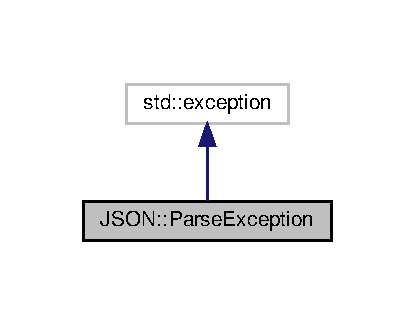
\includegraphics[width=201pt]{classJSON_1_1ParseException__inherit__graph}
\end{center}
\end{figure}


Collaboration diagram for J\+S\+ON\+::Parse\+Exception\+:
\nopagebreak
\begin{figure}[H]
\begin{center}
\leavevmode
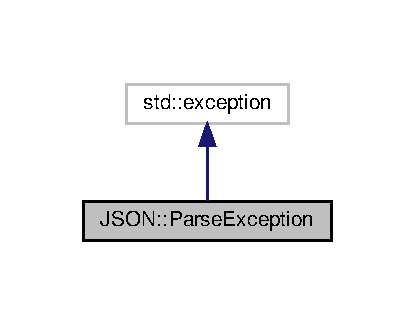
\includegraphics[width=201pt]{classJSON_1_1ParseException__coll__graph}
\end{center}
\end{figure}
\doxysubsection*{Public Member Functions}
\begin{DoxyCompactItemize}
\item 
\mbox{\Hypertarget{classJSON_1_1ParseException_af9bac4bf2265cc9c322ca0aa6cc95b29}\label{classJSON_1_1ParseException_af9bac4bf2265cc9c322ca0aa6cc95b29}} 
\mbox{\hyperlink{classJSON_1_1ParseException_af9bac4bf2265cc9c322ca0aa6cc95b29}{Parse\+Exception}} ()
\begin{DoxyCompactList}\small\item\em A \mbox{\hyperlink{classJSON_1_1ParseException}{Parse\+Exception}} osztály konstruktora. \end{DoxyCompactList}\item 
\mbox{\Hypertarget{classJSON_1_1ParseException_a8203c1af2b7f9eb83425ff04c4bd9e28}\label{classJSON_1_1ParseException_a8203c1af2b7f9eb83425ff04c4bd9e28}} 
\mbox{\hyperlink{classJSON_1_1ParseException_a8203c1af2b7f9eb83425ff04c4bd9e28}{$\sim$\+Parse\+Exception}} ()
\begin{DoxyCompactList}\small\item\em A \mbox{\hyperlink{classJSON_1_1ParseException}{Parse\+Exception}} osztály destruktora. \end{DoxyCompactList}\end{DoxyCompactItemize}


\doxysubsection{Detailed Description}
\begin{DoxyAuthor}{Authors}
Daniel\+Zettis, kormendiakos, M\+Zsolt97
\end{DoxyAuthor}
\begin{DoxyVersion}{Version}
2.\+0
\end{DoxyVersion}
\begin{DoxyDate}{Date}
2020/11/06
\end{DoxyDate}
Létrehozva\+: 2020/11/06 

The documentation for this class was generated from the following file\+:\begin{DoxyCompactItemize}
\item 
J\+S\+O\+N.\+h\end{DoxyCompactItemize}

%--- End generated contents ---

% Index
\backmatter
\newpage
\phantomsection
\clearemptydoublepage
\addcontentsline{toc}{chapter}{Index}
\printindex

\end{document}
